\subsection{Test 3}
\label{sec:test3}
% Results: data/TemporalEmail/resultados_dept1/cortes_fijos/c55d36031694cf39c08b/
% Requires graphicx and the existing natbib citation setup.
% Place quality_email_B10.pdf and quality_email_B40.pdf alongside the main
% manuscript, or add reports/ to its graphicspath.

We evaluate LSH-HLA on the Department 1 subset of the temporal email interaction dataset from a European research institution \citep{tempnetworkdata}. The complete department file contains 309 distinct users and 61,046 temporal interactions. We select the first 1,000 non-empty hourly layers, spanning the relative interval from day 0 at 00:00 to day 98 at 14:00 (exclusive). This interval contains 8,539 interactions involving 255 active users. All layers retain the same 309 nodes, with inactive users represented as isolated nodes. Repeated interactions are summed as edge weights, both within each layer and during graph aggregation, and message direction is discarded. The 1,366 hours without interactions in the selected interval are omitted from clustering. Days and hours are relative to the origin of the record, not calendar dates or local times.

The hourly layers are highly sparse: the median number of edges is four, 23.7\% of the layers contain a single edge, and the mean fraction of isolated nodes per layer is 96.5\%. This provides a different setting from Test 2 and motivates examining whether the regularizing behavior associated with $B$ persists under sparse temporal observations.

\subsubsection*{Experimental Protocol}
We retain the original aggregation strategy: candidate merges are restricted to clusters in the same bucket, with rehashing after aggregation during this phase; the method switches to global search when no eligible within-bucket pair remains. LSH-HLA uses five random graph projections generated with Erd\H{o}s--R\'enyi edge probability $p=0.5$. We evaluate $B=10$ and $B=40$ using ten runs each, with matched seeds 42--51. Parameter $B$ controls the discretization of each projection and is not the number of occupied multidimensional buckets.

To compare partitions at the same resolution, we use fixed cuts of $K\in\{5,10,20\}$ clusters rather than selecting a cut from the elbow of $q(C)$. For 1,000 layers, these cuts correspond to 995, 990, and 980 aggregation steps, respectively. These are exploratory resolutions, not estimated optimal cluster counts. The same complete hierarchy is reused for all three cuts, so the cuts do not constitute independent repetitions. Quality remains a descriptive measure and does not determine the cut.

The baseline performs exhaustive minimum-distance selection with bounded candidate storage and deterministic tie-breaking. It is executed once; its timing is therefore a single measurement, not a mean over ten runs. All LSH summaries use means and sample standard deviations over ten runs. Timings cover construction of the complete 999-merge hierarchy, excluding data loading, input preparation, and subsequent analysis. They do not measure early stopping at a fixed cut and refer specifically to the implementations evaluated here.

\subsubsection*{Computational Efficiency}
Table~\ref{tab:dept1_performance} summarizes computational performance. Relative to the baseline time of 3173.47 seconds, $B=10$ achieves a speedup of $1.54\times$ and a 35.0\% reduction in runtime, whereas $B=40$ achieves $1.43\times$ and a 30.1\% reduction. These ratios use the single baseline measurement and the mean LSH runtime.

\begin{table}[ht]
\centering
\begin{tabular}{lrr}
\hline
Method & Initial buckets & Time (s) \\
\hline
Baseline & -- & $3173.47$ \\
LSH-HLA, $B=10$ & $721.0\pm6.58$ & $2062.56\pm40.51$ \\
LSH-HLA, $B=40$ & $752.1\pm6.10$ & $2219.10\pm27.67$ \\
\hline
\end{tabular}
\caption{Runtime for complete hierarchies. LSH entries are means $\pm$ sample standard deviations across ten runs; the baseline is a single deterministic run.}
\label{tab:dept1_performance}
\end{table}

Increasing $B$ yields more occupied initial buckets and a higher mean runtime in this experiment.

\subsubsection*{Quality at Fixed Cuts}
Figure~\ref{fig:quality_email} displays the ten quality trajectories for each value of $B$, together with the baseline and the fixed cuts. Table~\ref{tab:dept1_fixed_quality} reports quality at those cuts. The baseline has higher $q(C)$ than either LSH configuration at every evaluated cut. Increasing $B$ from 10 to 40 produces small increases in mean quality: 0.0022, 0.0065, and 0.0079 for $K=5$, 10, and 20, respectively.

\begin{figure}[ht]
\centering
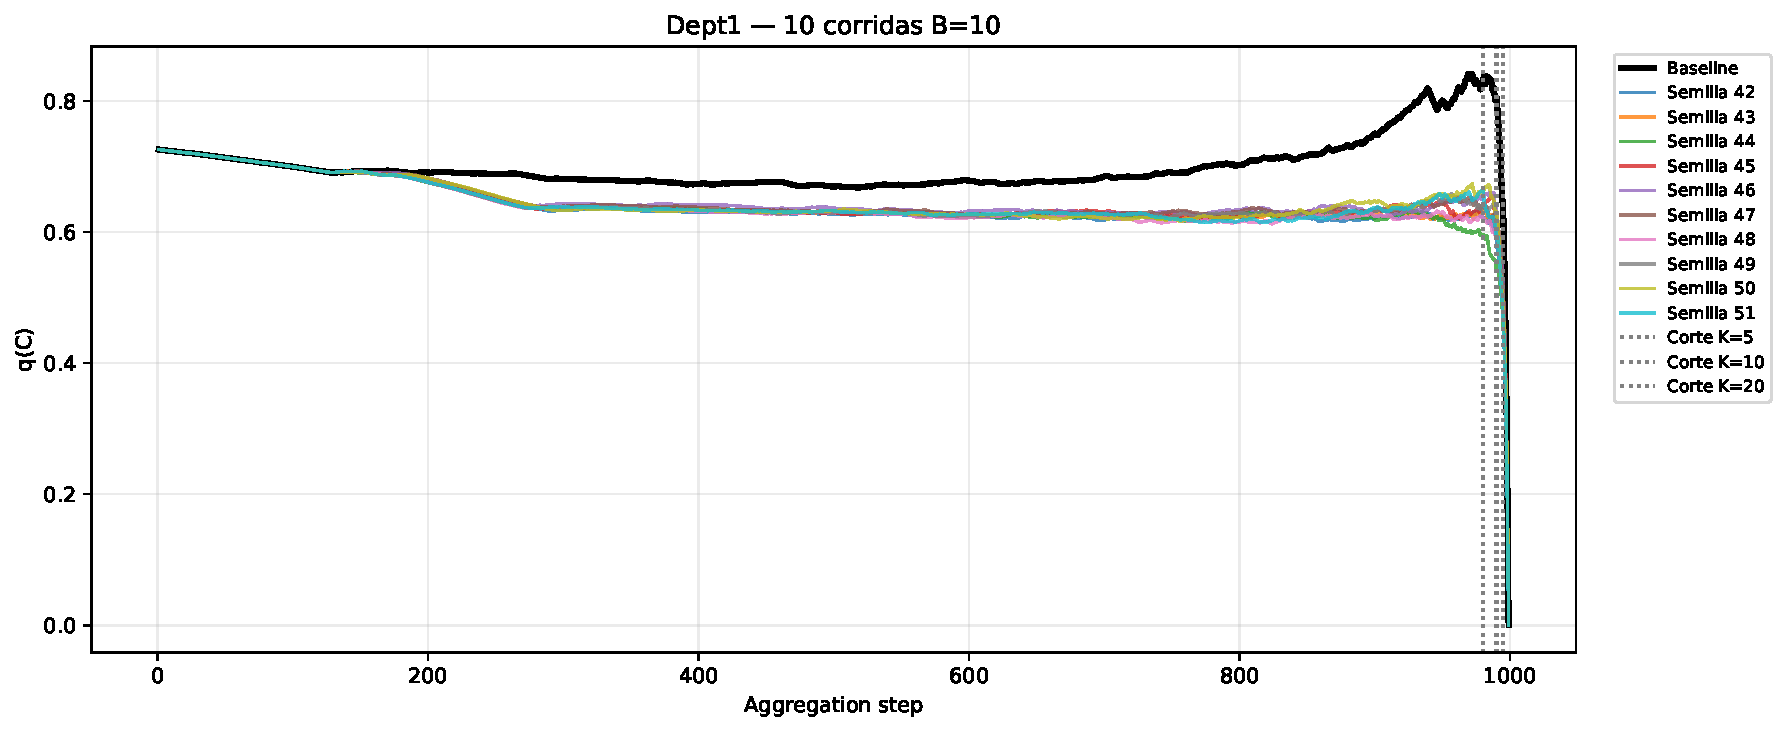
\includegraphics[width=0.95\linewidth]{quality_email_B10.pdf}\\[0.5em]
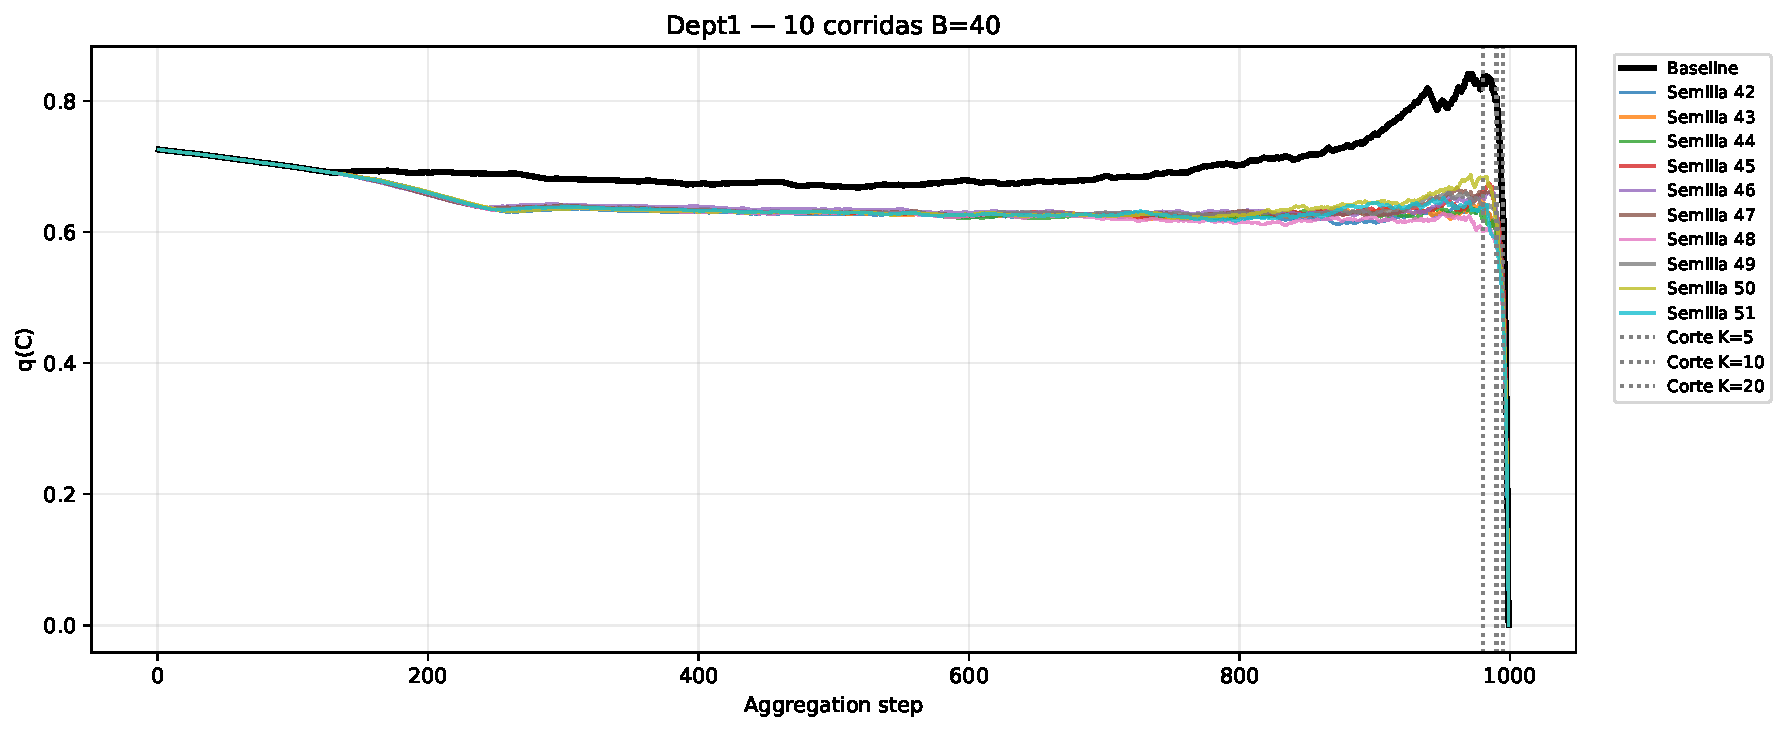
\includegraphics[width=0.95\linewidth]{quality_email_B40.pdf}
\caption{Ten LSH-HLA quality trajectories for $B=10$ (top) and $B=40$ (bottom), with the same baseline in each panel. Vertical lines mark the fixed cuts $K=5,10,20$; they are neither elbow estimates nor quality maxima.}
\label{fig:quality_email}
\end{figure}

\begin{table}[ht]
\centering
\begin{tabular}{rrrrr}
\hline
$K$ & Aggregation steps & Baseline $q$ & $B=10$: $q$ & $B=40$: $q$ \\
\hline
5 & 995 & 0.6332 & $0.4879\pm0.0228$ & $0.4900\pm0.0231$ \\
10 & 990 & 0.8057 & $0.6030\pm0.0271$ & $0.6095\pm0.0195$ \\
20 & 980 & 0.8326 & $0.6371\pm0.0219$ & $0.6450\pm0.0239$ \\
\hline
\end{tabular}
\caption{Quality at common fixed cuts. LSH entries summarize ten runs; baseline entries correspond to its single hierarchy.}
\label{tab:dept1_fixed_quality}
\end{table}

For matched seeds, $B=40$ yields higher quality in five of ten runs at $K=5$, five at $K=10$, and seven at $K=20$, with two ties at $K=5$ and one at $K=10$ within numerical tolerance. Its quality standard deviation decreases at $K=10$, but increases slightly at the other cuts. Consequently, the observed mean improvement is not accompanied by a consistent reduction in variability. The final decrease of quality to zero, when one cluster remains, follows from the definition of $q(C)$ and does not imply agreement between hierarchies.

\subsubsection*{Cluster Sizes and Membership Variability}
All evaluated partitions are strongly imbalanced, including the baseline (Table~\ref{tab:dept1_largest_cluster}). At $K=5$, the baseline places 996 layers in one cluster and leaves four singleton clusters. At $K=20$, its largest cluster still contains 964 layers. The mean largest-cluster sizes for LSH are 942.4 layers with $B=10$ and 945.5 with $B=40$ at this cut. Thus, fixing $K$ removes variability in cluster count by construction but does not produce balanced groups or establish membership stability.

\begin{table}[ht]
\centering
\begin{tabular}{rrrr}
\hline
$K$ & Baseline (\%) & $B=10$ (\%) & $B=40$ (\%) \\
\hline
5 & 99.60 & 99.27 & 99.29 \\
10 & 98.90 & 97.95 & 97.89 \\
20 & 96.40 & 94.24 & 94.55 \\
\hline
\end{tabular}
\caption{Percentage of layers in the largest cluster. LSH entries are averages over ten runs; the baseline is a single partition at each cut.}
\label{tab:dept1_largest_cluster}
\end{table}

As a descriptive membership comparison, we match clusters one-to-one to maximize the number of shared layers and divide that number by 1,000. Averaging over the 45 pairs of runs within each configuration gives 98.75\%, 96.48\%, and 91.42\% for $B=10$ at $K=5,10,20$, compared with 98.82\%, 96.45\%, and 91.94\% for $B=40$. These pairwise comparisons are not independent observations, and the score is not corrected for chance. In particular, it is dominated by agreement on the largest cluster: high overall overlap does not establish reproducibility of the smaller groups. The differences between the two values of $B$ are modest.

The current quality function assigns equal weight to each active cluster, irrespective of its number of constituent layers. A singleton therefore receives the same cluster-level weight as an aggregate containing most of the data. The high baseline quality must be interpreted alongside this size imbalance; it is not evidence by itself of a more meaningful temporal partition. Since the imbalance also appears without hashing, it cannot be attributed solely to the LSH approximation.

\subsubsection*{Local Patterns and Interpretation}
For an illustration chosen independently of quality, we inspect seed 42 at $K=10$. The largest cluster contains 972 layers with $B=10$ and 977 with $B=40$, and spans relative days 0--98 in both cases. Both configurations also recover the same eight-layer group, in which the undirected connection between users 157 and 185 appears in seven layers. This is a concrete recurring contact pattern retained across the two configurations, rather than evidence of general neighborhood preservation or stability across every seed. User identifiers are local to Department 1.

These observations support interpreting some small groups as recurring contacts or particular low-activity hours. They do not establish a clear decomposition into distinct temporal regimes: the dominant cluster retains most layers and most activity across the observation interval. Moreover, all users belong to the same department, so departmental composition cannot serve as external validation.

Overall, LSH-HLA reduces runtime, with $B=10$ providing the lower computational cost and $B=40$ providing only small improvements in mean quality. The regularizing behavior associated with $B$ in Test 2 is not consistently reproduced at these fixed cuts. The sparsity of the hourly layers provides a plausible context for this sensitivity, but the experiment does not isolate sparsity as its cause. As future work, the base method could be investigated using a quality function weighted by the number of constituent layers per cluster and strategies that merge buckets. Neither modification is applied in this experiment, and their effects on quality, stability, and runtime remain to be evaluated.
